\chapter{Chapter 4: Process Management}\label{ch-process-management}

\section{Introduction}\label{introduction}

In the previous chapters, we have discussed the topics that helped us to
understand the basics that are needed to initialize the environment for
a \lstinline!32-bit! protected mode kernel running on x86. Starting from
this chapter we are going to discuss the topics that belong to the
kernel itself, that is, the responsibilities of the kernel. We will
start with a quick look on the theories that are traditionally presented
on academic textbooks, then we move to the practical part in order to
implement these theories (or part of them) in 539kernel. A good place to
start from is \emph{process management}.

A kernel has multiple responsibilities, one of these responsibilities is
to manage the resources and make sure they are managed well. One
important resource of the computers is the time of the processor (AKA:
CPU time) which is the component that executes the code of software that
we would like to run on our machines. Process management is the the part
that studies how a kernel should manage and distribute CPU time among a
bunch of \emph{processes}.

\section{The Most Basic Work Unit: A
Process}\label{the-most-basic-work-unit-a-process}

\emph{Process} is the term which is used in operating systems literature
to describe a running program. In the previous chapters of this book we
have encountered the concept of the process multiple times and you may
recall from these encounters that every user-space software that we use
in our computers is a soulless sequence of bytes that are stored
somewhere in the hard disk. When we decide to use a specific software,
for example, the web browser, the first thing we do is to open it either
through double clicking on its icon in graphical user interfaces or
through writing its command in the shell. When we do that, the kernel is
needed to be called through a \emph{system call} and takes the
responsibility of ``opening'' this software, we can consider system
calls as functions which are provided by the kernel to expose its
services for the user-space software, one way of implementing system
calls is to use interrupts, exactly the same way that we have used with
BIOS.

However, there are multiple steps that are needed to be performed to
open the software, for example, reading its data from disk, but our
current focus is on process-related parts, eventually, the kernel
creates a new process for the software that we requested to open. The
kernel maintains a table of all system processes, each entry represents
a process and contains the information which is needed by the kernel to
manage the process, this data structure which stores a process
information is known as \emph{process control block} (PCB), so, the
processes table will have a process control block as an entry for each
process in the system.

Of course, the most important part of the process is the code of the
software that this process represents and its data, both data \footnote{We
  mean static data here, which are contained in the binary file of the
  software. While the data that are generated by the running process are
  not loaded from the binary file, instead they are created while the
  code is running (e.g.~local variables in the stack).} and code should
be loaded into memory, after that, its code can be executed by the
processor. We need to note that a process is an instance of a software,
in other words, one software can be opened more than one time with a
separated process for each one, for example, opening multiple windows of
the web browser on the same time, the software is one which is the web
browser and it is represented by the binary file which is stored in the
hard disk, but each opened window is a separated process and each
process' content is stored in the main memory. While the described
concept is well-known by the term ``process'', specially in the
literature, other terms can be used for the same concept, for example
\emph{task} and \emph{job} are other words which are used to point to
the same concept.

Each process is known to have a \emph{state}, when it is loaded to the
memory its state will be indicated by the kernel as \emph{ready} and can
be run anytime, when the CPU time is given to a process its state will
be \emph{running}. Also, the state of the process can be \emph{waiting},
an example of a situation where a process state is changed to waiting
state is when it performs I/O request (e.g.~read from the hard disk),
its state will be \emph{waiting} since it's waiting for the I/O device
to fulfill the request. The state information about a process is stored
in the process control block which is, as mentioned earlier, an entry in
the processes table.

Sometimes, a bunch of processes in a system need to communicate with
each other to share some data or tell each other to perform a specific
operation, this led to a broad topic known as \emph{inter-process
communication} (IPC) which provides mechanisms to make this type of
communication possible. The applications of \lstinline!IPC! is not
restricted to operating system kernels, they are used in distributed
computing for instance. One well known mechanism of \lstinline!IPC! is
\emph{shared memory}, that is, a region of the memory is made accessible
by more than one process, they can read and write to this region in
order to share data. The ability to write to same place by more than one
process can cause a problem known as \emph{race condition}, given a
shared variable, the situation which two or more processes try to change
the value of this variable at the same moment is known as race
condition. There are multiple solutions for this problem and this topic
is studied in a branch known \emph{concurrency control} which is a
shared topic by many applications, one of them is database management
systems (DBMS) which needs these mechanisms when two users try to update
the same row at the same time.

Processes are not the only entities that need to communicate, there is
another unit of work which is known as \emph{thread} and it can be
described as lightweight process. A process can have more than one
thread and when a software uses more than one thread to do its job, it
is described as \emph{multithreaded}. Threads are everywhere in our
usage of computers, and a world without them is unimaginable. For
example, when you use a text editor, the main thread of the software
lets you write your text, but when you click on save icon a separated
thread within the text editor's process is used to perform this
operation. Furthermore, another thread can be used for the spell checker
while you are typing. If all there functionalities were on one thread,
you will need to wait each one of them to finish in order to let you to
perform the other functionality, that is, the software without threads
is going to run sequentially while threads provide us concurrency within
one process. Threads and processes have many similarities, for example,
both of them are there to be executed, hence, they need to use the
processor and both of them need to be scheduled to give every one of
them time from the processor. In contrast to processes, threads run as a
part of same process and they share the same address space which makes
the communication between them much easier since they can reach the same
memory by default.

\section{The Basics of Multitasking}\label{the-basics-of-multitasking}

When we write a kernel, multiple design questions should be answered
\footnote{Remember the job of a kernelist!} and the part of process
management is not an exception of that. There are multiple well-known
answers for some basic design questions, each one of those answers tries
to solve a problem that faced the person who gave us this answer, for
example, one of well-known features of the modern operating systems is
\emph{multitasking} which is the successor of \emph{monotasking} and
both of them can be considered as answers for a design question in
operating systems. In multitasking environment, the system can run
multiple processes at the same time even if there is only one processor
available, while in monotasking environment, the system can run only one
process at a time until this process finishes its work or the user
closes it, only after that, another process can be run.

\subsection{Mutliprogramming \&
Time-Sharing}\label{mutliprogramming-time-sharing}

In the days of monotasking, we were facing a serious problem that led to
the birth of multitasking. It has been noticed that the processes tend
to have idle time, for example, when the process is waiting for the hard
disk to fetch some stored data, the process will be idle while it is
taking over the processor, that is, the processor is under the process'
control which is currently doesn't use the CPU time for something
useful, that means, in this case, we are wasting the valuable resource
of CPU time in waiting for some action to finish, we need to utilize the
processor as much as possible, and here came the solution of this
problem by letting the kernel to have a list of processes that are
\emph{ready} to run.

Assuming the machine has just one processor with one core, the CPU time
will be given to, say process \lstinline!A!, for some time and at some
point of running time the process \lstinline!A! requests from the disk
some data and due to that it becomes idle waiting for disk to respond.
Instead of keep the control of the processor under the process
\lstinline!A!, which is doing nothing but waiting right now, the kernel
suspends process \lstinline!A! and gives the CPU time to another ready
process, say process \lstinline!B!, this switching between two processes
is known as \emph{context switch}. The process \lstinline!B! is going to
use the processor while process \lstinline!A! is waiting for the disk to
respond. At some point, process \lstinline!B! will perform some action
that makes it idle which means that the kernel can switch to another
ready process and so on. This solution is known as
\emph{multiprogramming}. To sum it up, we have a list of ready
processes, choose one, give it the CPU time and wait for it until it
becomes idle, since it's waiting for something switch to another process
which is not idle an so on.

Better yet, multiprogramming has been extended to utilize the processor
more efficiently. Instead of waiting for the currently running process
to perform something which makes it idle, why don't we suspend it after
some period of running time whether it is idle or not and switch to
another process? This solution is known as \emph{time sharing} which is
with multiprogramming represent the scheme that modern operating systems
use for multitasking. In time sharing, a list of ready processes is
available for the kernel, in each unit of time, say for example, every
\lstinline!1! second (in practice, it is shorter) the currently running
process is suspended by the kernel and another process is given the CPU
time and so on.

\subsection{Process Scheduling}\label{process-scheduling}

You may recall from the previous chapter \ref{ch-progenitor} the system
timer which emits an interrupt every unit of time, this interrupt can be
used to implement time sharing in order to switch between the processes
of the system, of course the kernel needs an algorithm to choose which
process to run next, this kind of algorithms are known as
\emph{scheduling algorithms} and in general this part of the topic is
known as \emph{scheduling} in which we try to find the best way of
choosing the next process to run in order to satisfy our requirements.

The \emph{scheduler} is the part of the kernel that schedules the next
process by using some specific scheduling algorithm, that is, it decides
the next process to run based and performs the context switching. There
are many scheduling algorithms to deal with different requirements and
one of them is known as \emph{round-robin}. In this algorithm, each
process is given a fixed amount of CPU time known as \emph{quantum},
when the running process finishes its quantum the scheduler will be
called and the CPU time will be given to the next process in the list
until its quantum finishes and so on until the schedule reaches to the
end of the process list where it starts with the first process again.
The value of the quantum is decided by the kernelist, for example
\lstinline!50! milliseconds, which means each process will run
\lstinline!50! milliseconds then suspended to run the next one on the
list and so on.

\subsection{Process Context}\label{process-context}

As you know, when a process is executing, it can use the registers of
the processor (e.g. \lstinline!EAX!) to store its own data. Also, it may
change the values of segment registers in case it is running under a
system that employs segmented-memory instead of flat memory model.
Furthermore, the value of the instruction pointer \lstinline!EIP! will
contain an address which belong to the process' address space. All these
values that are related to a process and stored inside the registers of
the processor are known as \emph{process context}, another term which is
\emph{process state} may also be used in some places to mean the same
thing, but to not confuse this concept with the one that we have defined
the term ``state'' with previously, it is better to use the term process
context.

When a scheduler decides to change the currently running process, let's
call it \lstinline!A!, through a context switch, a copy of the context
of the process \lstinline!A! should be taken and stored somewhere, that
is, a snapshot of the last context of \lstinline!A! is taken before
switching to another process. By taking this snapshot, it will be easy
later to resume process \lstinline!A! by just loading its context to the
processor's register and jump to the the value of \lstinline!EIP! which
has been just loaded.

\subsection{Preemptive \& Cooperative
Multitasking}\label{preemptive-cooperative-multitasking}

Both multiprogramming and time-sharing solutions give us a type of
multitasking known as \emph{preemptive multitasking}, the processes are
forced by the kernel to give the CPU time to another process and no
process can take over the processor for the whole time. Another type of
multitasking is known as \emph{cooperative multitasking} (or
\emph{non-preemptive multitasking}), in this type the context switching
is not perform forcibly, instead, the currently running process should
cooperate and voluntarily tells the kernel when it should be suspended
and a context switch should be performed. One of the obvious problems of
this way, at least for the well-known workloads (e.g.~servers or
desktops), that a process, which runs a code that has been written by
someone we don't know, cannot be trusted. It simply may take over the
CPU time and never cooperate and give it up due to an error in the code
or even in purpose \footnote{You may ask who would use cooperative
  multitasking and give this big trust to the code of the software! In
  fact, the versions of Windows before 95 used this style of
  multitasking, also, Classic Mac OS used it. Why? You may ask, I don't
  know exactly, but what I know for sure is that humanity is in a
  learning process!}.

\section{Multitasking in x86}\label{multitasking-in-x86}

With the assistance of system timer, multitasking can be realized fully
by the kernel, that is, by the code. This type is known as
\emph{software multitasking}, the kernel itself is responsible for
storing the list of processes and their related information, also, it's
responsible for storing a snapshot of process context before performing
context switching and resuming this snapshot when the process is
resumed. On the other hand, In x86 some features are provided to handle
these things with the assistance of the processor itself, this type is
known as \emph{hardware multitasking}.

While hardware multitasking is available in x86, the modern operating
system kernels don't use it, instead, multitasking is implemented by the
kernel itself. One reason to take this decision is portability. Modern
kernels tend to run on more than one architecture and not only x86, by
using as little as possible of architecture's features it will be easier
to port a kernel to other architectures.

In this section, we are going to cover the basics of hardware
multitasking in x86 which are needed to initialize the environment to
make it work correctly, in the same way as \lstinline!GDT! with flat
memory model. Furthermore, I think knowing the other available options
is important, especially for kernelists. In 539kernel we are going to to
implement software multitasking as in modern kernels.

\subsection{Task-State Segments}\label{task-state-segments}

The most basic component of hardware multitasking in x86 is known as
\emph{task-state segment} (TSS) \footnote{In x86, the term task is used
  instead of process.} which is a segment in the memory as any other
code or data segment, it has what other segments have, a base address, a
limit and properties. The difference from code and data segments is that
\lstinline!TSS! is a system segment \footnote{In chapter \ref{ch-x86} we
  have seen that there are two types of segments in x86, application
  segments such as code, data and stack segment. And system segments and
  they are \lstinline!LDT! and \lstinline!TSS!.}, this segment stores
the context of a specific process.

In hardware multitasking, each process should has its own
\lstinline!TSS!, and each \lstinline!TSS! should has an entry in the
\lstinline!GDT! table, that is, \emph{TSS descriptor}. A special
register known as \emph{task register} should contain the segment
selector of the currently running process's \lstinline!TSS! descriptor,
the instruction \lstinline!ltr! is used to store a value in this
register.

\hypertarget{fig:tss}{
\begin{figure}
\centering
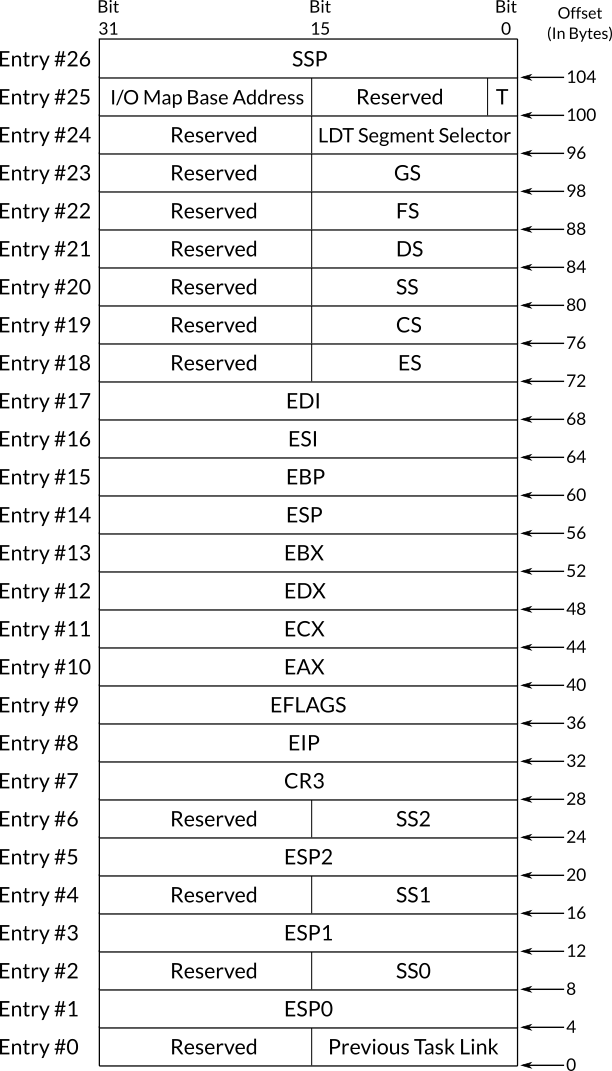
\includegraphics[width=0.45000\textwidth]{Figures/process-ch/tss.png}
\caption{Figure 1: The Structure of Task-State Segment}\label{fig:tss}
\end{figure}
}

Figure \protect\hyperlink{fig:tss}{1} shows the structure of a
task-state segment, as you can see, most of the fields are values of
registers while the others are out of our topic's range except for
previous task link which will be covered in a moment. You can see that
stack segment register and stack pointer register have four entries
instead of one, \lstinline!SS!, \lstinline!SS0!, \lstinline!SS1! and
\lstinline!SS2! for stack segment register. \lstinline!ESP!,
\lstinline!ESP0!, \lstinline!ESP1! and \lstinline!ESP2! for stack
pointer register. These fields point to the stack that should be used
when the process is in a specific privilege level, for example,
\lstinline!SS0:ESP0! will be used as the stack of the process when it
switches to privilege level \lstinline!0!, when it switches back to
privilege level \lstinline!3! the stack \lstinline!SS:ESP! will be used
instead, and the same is applicable to the other similar fields. If we
intend to implement software multitasking, the sole reason of defining
at least one \lstinline!TSS! is due to these fields, when a switch
between privilege levels occurs, the processor needs a \lstinline!TSS!
to use these fields from it in order to switch between stacks. This is
needed only when the system runs user-space code, that is, privilege
level \lstinline!3! code.

The structure of \lstinline!TSS! descriptor in \lstinline!GDT! table is
same as the segment descriptor that we have already explained in chapter
\ref{ch-x86}. The only difference is in the \emph{type field} which has
the static binary value \lstinline!010B1! in \lstinline!TSS! descriptor
where \lstinline!B! in this value is known as \lstinline!B! flag, or
\emph{busy flag} which should be \lstinline!1! when the process that
this TSS descriptor represents is active and \lstinline!0! when it is
inactive.

\subsection{Context Switching in x86}\label{context-switching-in-x86}

One way of switching from a process to another \footnote{In x86, context
  switch is known as task switch.} in x86 hardware multitasking is to
call or jump to TSS descriptor in \lstinline!GDT!, assume that the
system timer caused the call of the scheduler which selects process
\lstinline!A! as the next process to run, the scheduler can cause
context switch by using the instructions \lstinline!call! or
\lstinline!jmp! and the operand should be the segment selector of
\lstinline!A!'s TSS descriptor. In this way, the processor is going to
take a copy of currently running process (call it \lstinline!B!) and
store it in \lstinline!B!'s own \lstinline!TSS!, then the values in
\lstinline!A!'s TSS will be loaded into the processor registers and then
execution of \lstinline!A! begins.

Another way of context switching in x86 hardware multitasking is to call
or jump to a task gate. In chapter \ref{ch-x86}, when we discussed the
descriptors of \lstinline!IDT!, we have said that one type of descriptor
that can be defined is a task gate descriptor. This kind of descriptors
is considered as a separated process by the processor, when we jump or
call a task gate, the previously explained mechanism of task switching
will be performed. Task gates can also be defined in \lstinline!GDT! and
\lstinline!LDT!. In the \lstinline!IDT! table of 539kernel we have
chosen to not define the interrupts as task gates, we don't want to
perform a context switch with each interrupt.

When a process is called instead of jumped to, eventually, it should
return to the caller process by using the instruction \lstinline!iret!,
for the processor, to be able to decide which task is the caller, the
previous task link field of the callee's \lstinline!TSS! will be updated
to contain the segment selector of the caller process. In this way, when
\lstinline!iret! instruction is executed, it will be easy to know to
which process the processor should switch back to.

\section{Process Management in
539kernel}\label{process-management-in-539kernel}

The final result of this section is what I call version \lstinline!T! of
539kernel which has a basic multitasking capability. The multitasking
style that we are going to implement is time-sharing multitasking. Also,
instead of depending on x86 features to implement multitasking in
539kernel, a software multitasking will be implemented. The final
\lstinline!Makefile! of version \lstinline!T! is provided in the last
subsection, however, if you wish to build and run the kernel
incrementally after each change on the progenitor you can refer to that
\lstinline!Makefile! and add only the needed instructions to build the
not ready yet version \lstinline!T! that you are building. For example,
as you will see in a moment new files \lstinline!screen.c! and
\lstinline!screen.h! will be added in version \lstinline!T! as a first
increment, to run the kernel after adding them you need to add the
command to compile this new file and link it with the previous files,
you can find these commands in the last version of \lstinline!Makefile!
as we have said before.

Our first step of this implementation is to setup a valid task-state
segment, while 539kernel implements a software multitasking, a valid TSS
is needed. As we have said earlier, it will not be needed in our current
stage but we will set it up anyway. Its need will show up when the
kernel lets user-space software to run. After that, basic data
structures for process table and process control block are implemented.
These data structures and their usage will be as simple as possible
since we don't have any mean for dynamic memory allocation, yet! After
that, the scheduler can be implemented and system timer's interrupt can
be used to enforce preemptive multitasking by calling the scheduler
every period of time. The scheduler uses round-robin algorithm to choose
the next process that will use the CPU time, and the context switching
is performed after that. Finally, we are going to create a number of
processes to make sure that everything works fine.

Before getting started in the plan that has been just described, we need
to organize our code a little bit since it's going to be larger starting
from this point. New two files should be created, \lstinline!screen.c!
and its header file \lstinline!screen.h!. We move the printing functions
that we have defined in the progenitor and their related global
variables to \lstinline!screen.c! and their prototypes should be in
\lstinline!screen.h!, so, we can \lstinline!include! the latter in other
C files when we need to use the printing functions. The following is the
content of \lstinline!screen.h!.

\begin{lstlisting}[language=C]
volatile unsigned char *video;

int nextTextPos;
int currLine;

void screen_init();
void print( char * );
void println();
void printi( int );
\end{lstlisting}

As you can see, a new function \lstinline!screen_init! has been
introduced while the others are same as the ones that we already wrote.
The function \lstinline!screen_init! will be called by the kernel once
it starts running, the function initializes the values of the global
variables \lstinline!video!, \lstinline!nextTextPos! and
\lstinline!currLine!. Its code is the following and it should be in
\lstinline!screen.c!, of course in the beginning of this file,
\lstinline!screen.h! should be included by using the line
\lstinline!#include "screen.h"!.

\begin{lstlisting}[language=C]
void screen_init()
{
    video = 0xB8000;
    nextTextPos = 0;
    currLine = 0;
}
\end{lstlisting}

Nothing new in here, just some organizing. Now, the prototypes and
implementations of the functions \lstinline!print!, \lstinline!println!
and \lstinline!printi! should be removed from \lstinline!main.c!.
Furthermore, the global variables \lstinline!video!,
\lstinline!nextTextPos! and \lstinline!currLine! should also be removed
from \lstinline!main.c!. Now, the file \lstinline!screen.h! should be
included in \lstinline!main.c! and in the beginning of the function
\lstinline!kernel_main! the function \lstinline!screen_init! should be
called.

\subsection{Initializing the Task-State
Segment}\label{initializing-the-task-state-segment}

Setting TSS up is too simple. First we know that the TSS itself is a
region in the memory (since it is a segment), so, let's allocate this
region of memory. The following should be added at end of
\lstinline!starter.asm!, even after including the files
\lstinline!gdt.asm! and \lstinline!idt.asm!. In the following a label
named \lstinline!tss! is defined, and inside this region of memory,
which its address is represented by the label \lstinline!tss!, we put a
doubleword of \lstinline!0!, recall that a word is \lstinline!2! bytes
while a double-word is \lstinline!4! bytes. So, our \lstinline!TSS!
contains nothing but a bunch of zeros.

\begin{lstlisting}
tss:
    dd 0
\end{lstlisting}

As you may recall, each \lstinline!TSS! needs an entry in the
\lstinline!GDT! table, after defining this entry, the TSS's segment
selector can be loaded into the task register. Then the processor is
going to think that there is one process (one \lstinline!TSS! entry in
\lstinline!GDT!) in the environment and it is the current process (The
segment selector of this \lstinline!TSS! is loaded into task register).
Now, let's define the TSS entry in our \lstinline!GDT! table. In the
file \lstinline!gdt.asm! we add the following entry at the end of the
label \lstinline!gdt!. You should not forget to modify the size of
\lstinline!GDT! under the label \lstinline!gdt_size_in_bytes! under
\lstinline!gdtr! since the sixth entry has been added to the table.

\begin{lstlisting}
tss_descriptor: dw tss + 3, tss, 0x8900, 0x0000
\end{lstlisting}

Now, let's get back to \lstinline!starter.asm! in order to load TSS'
segment selector into the task register. In \lstinline!start! routine
and below the line \lstinline!call setup_interrupts! we add the line
\lstinline!call load_task_register! which calls a new routine named
\lstinline!load_task_register! that loads the task register with the
proper value. The following is the code of this routine that can be
defined before the line \lstinline!bits 32! in \lstinline!starter.asm!.

\begin{lstlisting}
load_task_register:
    mov ax, 40d
    ltr ax
    
    ret
\end{lstlisting}

As you can see, it's too simple. The index of TSS descriptor in
\lstinline!GDT! is
\lstinline!40 = (entry 6 * 8 bytes) - 8 (since indexing starts from 0)!.
So, the value \lstinline!40! is moved to the register \lstinline!AX!
which will be used by the instruction \lstinline!ltr! to load the value
\lstinline!40! into the task register.

\subsection{The Data Structures of
Processes}\label{the-data-structures-of-processes}

When we develop a user-space software and we don't know the size of the
data that this software is going to store while it's running, we usually
use dynamic memory allocation, that is, regions of memory are allocated
at run-time in case we need to store more data that we didn't know that
it will be needed to be stored. We have encountered the run-time stack
previously, and you may recall that this region of memory is dedicated
for local variables, parameters and some information that make function
invocation possible.

The other region of a process is known as run-time heap, which is
dedicated for the data that we decided to store in memory while the
software is running. In C, for instance, the function \lstinline!malloc!
is used to allocate bytes from the run-time heap and maintains
information about free and used space of the heap so in the next use of
this function the allocation algorithm can decide which region should be
allocated based on the required bytes to allocate.

This part that allocates memory dynamically (inside run-time heap) and
manages the related stuff is known as \emph{memory allocator} and one of
well-known allocators is Doug Lea's memory allocator. For programming
languages that run the program by using a virtual machine, like Java and
C\#, or by using interpreters like PHP and Python, they usually provide
their users an automatic dynamic memory allocation instead of the manual
memory allocation which is used by languages such as C, that is, the
programmer of these languages don't need to explicitly call a function
(such as \lstinline!malloc!) to allocate memory in the heap at run-time,
instead, the virtual machine or the interpreter allocates dynamic memory
by itself and frees the region of the heap that are not used anymore
through a mechanism known as \emph{garbage collection}.

For those who don't know, in static memory allocation, the size of data
and where will it be stored in the memory are known in compiling time,
global variables and local variables are examples of objects that we use
static memory allocation for them. In dynamic memory allocation, we
cannot decide in compiling time the size of the data or whether it will
be stored in the first place, these important information will only be
known while the software is running, that is, in run-time. Due to that,
we need to use dynamic memory allocation for them since this type of
allocation doesn't require these information in the compiling time.

Processes table is an example of data structures (objects) that we can't
know its size in compile-time and this information can be only decided
while the kernel is running. Take your current operating system as an
example, you can run any number of processes (to some limit of course)
and all of them will have an entry in the processes table \footnote{We
  already know that keeping an entry of a process in the processes table
  is important for the scheduling process and other related processes
  stuff.}, maybe your system is running just two processes right now but
you can run more and more without the need of recompiling the kernel in
order to increase the size of processes table.

That's possible due to using dynamic memory allocation when a new
process is created during run-time and that's by dynamically allocating
a space in the run-time heap through the memory allocator for this the
entry of this new process. When this process finishes its job (e.g.~the
user closes the application), the memory region that is used to store
its entry in processes table is marked as free space so it can be used
to store something else in the future, for example, the entry of another
process.

In our current situation, we don't have any means of dynamic memory
allocation in 539kernel, this topic will be covered when we start
discussing memory management. Due to that, our current implementations
of processes table and process control block are going to use static
memory allocation through global variables. That of course, restricts us
from creating a new process on-the-fly, that is, at run-time. But our
current goal is to implement a basic multitasking that will be extended
later. To start our implementation, we need to create new two files,
\lstinline!process.c! and its header file \lstinline!process.h!. Any
function or data structure that is related to processes should belong to
these file.

\subsubsection{Process Control Block}\label{process-control-block}

A process control block (PCB) is an entry in the processes table, it
stores the information that are related to a specific process, the state
and context of the process are examples of these information. In
539kernel, there are two possible states for a process, either a process
is \emph{running} or \emph{ready}. When a context switch is needed to be
performed, the context of the currently running process, which will be
suspended, should be stored on its own PCB. Based on our previous
discussions, the context of the process in 539kernel consists the values
which were stored in the processor's registers before suspending the
process.

Each process in 539kernel, as in most modern kernels, has a unique
identifier known as \emph{process id} or PID for short, this identifier
is also stored in the PCB of the process. Now, let's define the general
structure of PCB and its components in 539kernel. These definitions
should reside in \lstinline!process.h!.

\begin{lstlisting}[language=C]
typedef enum process_state { READY, RUNNING } process_state_t;

typedef struct process_context
{
    int eax, ecx, edx, ebx, esp, ebp, esi, edi, eip;
} process_context_t;

typedef struct process
{
    int pid;
    process_context_t context;
    process_state_t state;
    int *base_address;
} process_t;
\end{lstlisting}

As you can see, we start by a type known as \lstinline!process_state_t!,
any variable that has this type may have two possible values,
\lstinline!READY! or \lstinline!RUNNING!, they are the two possible
states of a process and this type will be used for the state field in
PCB definition.

Next, the type \lstinline!process_context_t! is defined. It represents
the context of a process in 539kernel and you can see it is a C
structure that intended to store a snapshot of x86 registers that can be
used by a process.

Finally, the type \lstinline!process_t! is defined which represents a
process control block, that is, an entry in the processes table. A
variable of type \lstinline!process_t! represents one process in
539kernel environment. Each process has a \lstinline!pid! which is its
unique identifier. A \lstinline!context! which is the snapshot of the
environment before suspending the process. A \lstinline!state! which
indicates whether a process is \lstinline!READY! to run or currently
\lstinline!RUNNING!. And finally, a \lstinline!base_address! which is
the memory address of the process' code starting point (think of
\lstinline!main()! in C), that is, when the kernel intend to run a
process for the first time, it should jump to the
\lstinline!base_address!, in other words, set \lstinline!EIP! to
\lstinline!base_address!.

\subsubsection{Processes Table}\label{processes-table}

In the current case, as we mentioned earlier, we are going to depend on
static memory allocation since we don't have any way to employ dynamic
memory allocation. Due to that, our processes table will be too simple,
it is an array of type \lstinline!process_t!. Usually, more advanced
data structure is used for the processes list based on the requirements
which are decided by the kernelist, \emph{linked list data structure} is
a well-known choice. The following definition should reside in
\lstinline!process.h!. Currently, the maximum size of 539kernel
processes table is \lstinline!15! processes, feel free to increase it
but don't forget, it will, still, be a static size.

\begin{lstlisting}[language=C]
process_t *processes[ 15 ];
\end{lstlisting}

\subsection{Process Creation}\label{process-creation}

Now, we are ready to write the function that creates a new process in
539kernel. Before getting started in implementing the required
functions, we need to define their prototypes and some auxiliary global
variables in \lstinline!process.h!.

\begin{lstlisting}[language=C]
int processes_count, curr_pid;

void process_init();
void process_create( int *, process_t * );
\end{lstlisting}

The first global variable \lstinline!processes_count! represents the
current number of processes in the environment, this value will become
handy when we write the code of the scheduler which uses round-robin
algorithm, simply, whenever a process is created in 539kernel, the value
of this variable is increased and since deleting a process will not be
implemented for the sake of simplicity, the value of this variable will
not be decreased anywhere in the current code of 539kernel.

The global variable \lstinline!curr_pid! contains the next available
process identifier that can be used for the next process that will be
created. The current value of this variable is used when creating a new
process and its value is increased by one after completing the creation.

The function \lstinline!process_init! is called when the kernel starts,
and it initializes the process management subsystem by just initializing
the two global variables that we mentioned.

The function \lstinline!process_create! is the one that creates a new
process in 539kernel, that is, it is equivalent to \lstinline!fork! in
Unix systems. As you can see, it takes two parameters, the first one is
a pointer to the base address of the process, that is, the starting
point of the process' code. The second parameter is a pointer to the
process control block, as we have said, currently, we use static memory
allocation, therefore, each new PCB will be either stored in the memory
as a local or global variables, so, for now, the caller is responsible
for allocating a static memory for the PCB and passing its memory
address in the second parameter. In the normal situation, the memory of
a PCB is allocated dynamically by the creation function itself, but
that's a story for another chapter. The following is the content of
\lstinline!process.c! as we have described.

\begin{lstlisting}[language=C]
#include "process.h"

void process_init()
{
    processes_count = 0;
    curr_pid = 0;
}

void process_create( int *base_address, process_t *process )
{   
    process->pid = curr_pid++;
    
    process->context.eax = 0;
    process->context.ecx = 0;
    process->context.edx = 0;
    process->context.ebx = 0;
    process->context.esp = 0;
    process->context.ebp = 0;
    process->context.esi = 0;
    process->context.edi = 0;
    process->context.eip = base_address;
    
    process->state = READY;
    process->base_address = base_address;
    
    processes[ process->pid ] = process;
    
    processes_count++;
}
\end{lstlisting}

In \lstinline!process_create!, a new process identifier is assigned to
the new process. Then the context is initialized, this structure will be
used later in context switching, either by copying the values from the
processor to the structure or vice versa. Since the new process has not
been run yet, hence, it didn't set any value to the registers, then we
initialize all general purpose registers with \lstinline!0!, later on,
when this process runs and the scheduler decides to suspend it, the
values that this process wrote on the real registers will be copied in
here. The structure field of program counter \lstinline!EIP! is
initialized with the starting point of the process' code, in this way we
can make sure that when the scheduler decides to run this process, it
loads the correct value to the register \lstinline!EIP!.

After initializing the context, the state of the process is set as
\lstinline!READY! to run and the base address of the process is stored
in a separate field. Then, the freshly-created PCB is added to the
processes list and finally the number of processes in the system is
increased by one.

That' all we need for now to implement multitasking, in real cases,
there will be usually more process states such as \emph{waiting}, the
data structures are allocated dynamically to make it possible to create
virtually any number of processes, the PCB may contains more fields and
more functions to manipulate processes table (e.g.~delete process) are
implemented. However, our current implementation, though too simple, it
is enough as a working foundation. Now, in \lstinline!main.c!, the
header file \lstinline!process.h! is needed to be included, and the
function \lstinline!process_init! should be called in the beginning of
the kernel, after the line \lstinline!screen_init();!.

\subsection{The Scheduler}\label{the-scheduler}

Right now, we have all needed components to implement the core of
multitasking, that is, the scheduler. As mentioned multiple times
before, round-robin algorithm is used for 539kernel's scheduler.

Let's present two definitions to make our next discussion more clear.
The term \emph{current process} means the process that is using the
processor right now, at some point of time, the system timer emits an
interrupt which suspends the current process and calls the kernel to
handle the interrupt, In this case the kernel is going to call the
scheduler, at this point of time, we keep the same term for the process
which was running right before calling the kernel to handle the
interrupt, we call it the current process. By using some algorithm, the
scheduler chooses the \emph{next process}, that is, the process that
will run after the scheduler finishes its work and the kernel returns
the processor to the processes. After choosing the next process,
performing the context switching and jumping to the process code, this
chosen process will be the current process instead of the suspended one,
and it will be the current process until the next run of the scheduler
and so on.

Now, we are ready to implement the scheduler, let's create a new file
\lstinline!scheduler.c! and its header file \lstinline!scheduler.h! for
the new code. The following is the content of the header file.

\begin{lstlisting}[language=C]
#include "process.h"

int next_sch_pid, curr_sch_pid;

process_t *next_process;

void scheduler_init();
process_t *get_next_process();
void scheduler( int, int, int, int, int, int, int, int, int );
void run_next_process();
\end{lstlisting}

First, \lstinline!process.h! is included since we need to use the
structure \lstinline!process_t! in the code of the scheduler. Then three
global variables are defined, the global variable
\lstinline!next_sch_pid! stores the PID of the next process that will
run after next system timer interrupt, while \lstinline!curr_sch_pid!
stores the PID of the current process. The global variable
\lstinline!next_process! stores a reference to the PCB of the next
process, this variable will be useful when we want to move the control
of the processor from the kernel to the next process which is the job of
the function \lstinline!run_next_process!.

The function \lstinline!scheduler_init! sets the initial values of the
global variables, same as \lstinline!process_init!, it will be called
when the kernel starts.

The core function is \lstinline!scheduler! which represents 539kernel's
scheduler, this function will be called when the system timer emits its
interrupt. It chooses the next process to run with the help of the
function \lstinline!get_next_process!, performs context switching by
copying the context of the current process from the registers to the
memory and copying the context of the next process from the memory to
the registers. Finally, it returns and \lstinline!run_next_process! is
called in order to jump the the next process' code. In
\lstinline!scheduler.c!, the file \lstinline!scheduler.h! should be
included to make sure that everything works fine. The following is the
implementation of \lstinline!scheduler_init!.

\begin{lstlisting}[language=C]
void scheduler_init()
{
    next_sch_pid = 0;
    curr_sch_pid = 0;
}
\end{lstlisting}

It's too simple function that initializes the values of the global
variables by setting the PID \lstinline!0! to both of them, so the first
process that will be scheduled by 539kernel is the process with PID
\lstinline!0!.

Next, is the definition of \lstinline!get_next_process! which implements
round-robin algorithm, it returns the PCB of the process that should run
right now and prepare the value of \lstinline!next_sch_pid! for the next
context switching by using round-robin policy.

\begin{lstlisting}[language=C]
process_t *get_next_process()
{
    process_t *next_process = processes[ next_sch_pid ];
    
    curr_sch_pid = next_sch_pid;
    next_sch_pid++;
    next_sch_pid = next_sch_pid % processes_count;
    
    return next_process;
}
\end{lstlisting}

Too simple, right! \footnote{Could be simpler, but the readability is
  more important here.} If you haven't encountered the symbol
\lstinline!%! previously, it represents an operation called
\emph{modulo} which gives the remainder of division operation, for
example, \lstinline!4 % 2 = 0! because the reminder of dividing
\lstinline!4! on \lstinline!2! is \lstinline!0!, but
\lstinline!5 % 2 = 1! because \lstinline!5 / 2 = 2! and remainder is
\lstinline!1!, so, \lstinline!5 = ( 2 * 2 ) + 1 (the remainder)!.

In modulo operation, any value \lstinline!n! that has the same position
of \lstinline!2! in the previous two examples is known as
\emph{modulus}. For instance, the modulus in \lstinline!5 % 3! is
\lstinline!3! and the modulus in \lstinline!9 % 10! is \lstinline!10!
and so on. In some other places, the symbol \lstinline!mod! is used to
represent modulo operation instead of \lstinline!%!.

The interesting thing about modulo that its result value is always
between the range \lstinline!0! and \lstinline!n - 1! given that
\lstinline!n! is the modulus. For example, let the modulus be
\lstinline!2!, and we perform the following modulo operation
\lstinline!x % 2! where \lstinline!x! can be any number, the possible
result values of this operation are only \lstinline!0! or \lstinline!1!.
Using this example with different values of \lstinline!x! gives us the
following results, \lstinline!0 % 2 = 0!, \lstinline!1 % 2 = 1!,
\lstinline!2 % 2 = 0!, \lstinline!3 % 2 = 1!, \lstinline!4 % 2 = 0!,
\lstinline!5 % 2 = 1!, \lstinline!6 % 2 = 0! and so on to infinity!

As you can see, modulo gives us a cycle that starts from \lstinline!0!
and ends at some value that is related to the modulus and starts all
over again with the same cycle given an ordered sequence of values for
\lstinline!x!, sometimes the analog clock is used as metaphor to
describe the modulo operation. However, in mathematics a topic known as
\emph{modular arithmetic} is dedicated to the modulo operation. You may
noticed that modulo operation can be handy to implement round-robin
algorithm.

Let's get back to the function \lstinline!get_next_process! which
chooses the next process to run in a round-robin fashion. As you can
see, it assumes that the PID of the next process can be found directly
in \lstinline!next_sch_pid!. By using this assumption it fetches the PCB
of this process to return it later to the caller. After that, the value
of \lstinline!curr_sch_pid! is updated to indicate that, right now, the
current process is the one that we just selected to run next. The next
two lines are the core of the operation of choosing the next process to
run, it prepares which process will run when next system timer interrupt
occurs.

Assume that the total number of processes in the system is
\lstinline!4!, that is, the value of \lstinline!processes_count! is
\lstinline!4!, and assume that the process that will run in the current
system timer interrupt has the PID \lstinline!3!, that is
\lstinline!next_sch_pid = 3!, PIDs in 539kernel start from
\lstinline!0!, that means there is no process with PID \lstinline!4! in
our example and process \lstinline!3! is the last one.

In line \lstinline!next_sch_pid++! the value of the variable will be
\lstinline!4!, and as we mentioned, the last process is \lstinline!3!
and there is no such process \lstinline!4!, that means we should start
over the list of processes and runs process \lstinline!0! in the next
cycle, we can do that simply by using modulo on the new value of
\lstinline!next_sch_pid! with the modulus \lstinline!4! which is the
number of processes in the system \lstinline!process_count!, so,
\lstinline!next_sch_pid = 4 % 4 = 0!. In the next cycle, process
\lstinline!0! will be chosen to run, the value of
\lstinline!next_sch_pid! will be updated to \lstinline!1! and since it
is lesser than \lstinline!process_count! it will be kept for the next
cycle. After that, process \lstinline!1! will run and the next to run
will be \lstinline!2!. Then process \lstinline!2! will run and next to
run is \lstinline!3!. Finally, the same situation that we started our
explanation with occurs again and process \lstinline!0! is chosen to run
next. The following is the code of the function \lstinline!scheduler!.

\begin{lstlisting}[language=C]
void scheduler( int eip, int edi, int esi, int ebp, int esp, int ebx, int edx, int ecx, int eax )
{
    process_t *curr_process;
    
    // ... //
    
    // PART 1
    
    curr_process = processes[ curr_sch_pid ];
    next_process = get_next_process();
    
    // ... //
    
    // PART 2

    if ( curr_process->state == RUNNING )
    {
        curr_process->context.eax = eax;
        curr_process->context.ecx = ecx;
        curr_process->context.edx = edx;
        curr_process->context.ebx = ebx;
        curr_process->context.esp = esp;
        curr_process->context.ebp = ebp;
        curr_process->context.esi = esi;
        curr_process->context.edi = edi;
        curr_process->context.eip = eip;
    }
    
    curr_process->state = READY;
    
    // ... //
    
    // PART 3
    
    asm( "  mov %0, %%eax;  \
            mov %0, %%ecx;  \
            mov %0, %%edx;  \
            mov %0, %%ebx;  \
            mov %0, %%esi;  \
            mov %0, %%edi;" 
            : : "r" ( next_process->context.eax ), "r" ( next_process->context.ecx ), "r" ( next_process->context.edx ), "r" ( next_process->context.ebx ),
                "r" ( next_process->context.esi ), "r" ( next_process->context.edi ) );
    
    next_process->state = RUNNING;
}
\end{lstlisting}

I've commented the code to divide it into three parts for the sake of
simplicity in our discussion. The first part is too simple, the variable
\lstinline!curr_process! is assigned to a reference to the current
process which has been suspended due to the system timer interrupt, this
will become handy in part \lstinline!2! of scheduler's code, we get the
reference to the current process before calling the function
\lstinline!get_next_process! because, as you know, this function changes
the variable of current process' PID (\lstinline!curr_sch_pid!) from the
suspended one to the next one \footnote{And that's why the global
  variables are considered evil.}. After that, the function
\lstinline!get_next_process! is called to obtain the PCB of the process
that will run this time, that is, the next process.

As you can see, \lstinline!scheduler! receives nine parameters, each one
of them has a name same as one of the processor's registers. We can tell
from these parameters that the function \lstinline!scheduler! receives
the context of the current process before being suspended due to system
timer's interrupt. For example, assume that process \lstinline!0! was
running, after the quantum finished the scheduler is called, which
decides that process \lstinline!1! should run next. In this case, the
parameters that have been passed to the scheduler represent the context
of process \lstinline!0!, that is, the value of the parameter
\lstinline!EAX! will be same as the value of the register
\lstinline!EAX! that process \lstinline!0! set at some point of time
before being suspended. How did we get these values and pass them as
parameters to \lstinline!scheduler!? This will be discussed later.

In part \lstinline!2! of scheduler's code, the context of the suspended
process, which \lstinline!curr_process! represents it right now, is
copied from the processor into its own PCB by using the passed
parameter. Storing current process' context into its PCB is simple as
you can see, we just store the passed values in the fields of the
current process structure. These values will be used later when we
decide to run the same process. Also, we need to make sure that the
current process is really running by checking its \lstinline!state!
before copying the context from the processor to the PCB. At the end,
the \lstinline!state! of the current process is switched from
\lstinline!RUNNING! to \lstinline!READY!.

Part \lstinline!3! performs the opposite of part \lstinline!2!, it uses
the PCB of the next process to retrieve its context before the last
suspension, then this context will be copied to the registers of the
processor. Of course, not all of them are being copied to the processor,
for example, the program counter \lstinline!EIP! cannot be written to
directly, we will see later how to deal with it. Also, the registers
that are related to the stack, \lstinline!ESP! and \lstinline!EBP! were
skipped in purpose. As a last step, the \lstinline!state! of the next
process is changed from \lstinline!READY! to \lstinline!RUNNING!. The
following is the code of \lstinline!run_next_process! which is last
function remains in \lstinline!scheduler.c!.

\begin{lstlisting}[language=C]
void run_next_process()
{
    asm( "  sti;            \
            jmp *%0" : : "r" ( next_process->context.eip ) );
}
\end{lstlisting}

It is a simple function that executes two assembly instructions. First
it enables the interrupts via the instruction \lstinline!sti!, then it
jumps to the memory address which is stored in the \lstinline!EIP! of
next process' PCB. The purpose of this function will be discussed after
a short time.

To make everything runs properly, \lstinline!scheduler.h! need to be
included in \lstinline!main.c!, note that, when we include
\lstinline!scheduler.h!, the line which includes \lstinline!process.h!
should be remove since \lstinline!scheduler.h! already includes it.
After that, the function \lstinline!scheduler_init! should be called
when initializing the kernel, say after the line which calls
\lstinline!process_init!.

\subsubsection{Calling the Scheduler}\label{calling-the-scheduler}

``So, how the scheduler is being called'' you may ask. The answer to
this question has been mentioned multiple times before. When the system
timer decides that it is the time to interrupt the processor, the
interrupt \lstinline!32! is being fired, this point of time is when the
scheduler is being called. In each period of time the scheduler will be
called to schedule another process and gives it CPU time.

In this part, we are going to write a special interrupt handler for
interrupt \lstinline!32! that calls 539kernel's scheduler. First we need
to add the following lines in the beginning of \lstinline!starter.asm!
\footnote{I'm about to regret that I called this part of the kernel the
  starter! obviously it's more than that!} after
\lstinline!extern interrupt_handler!.

\begin{lstlisting}
extern scheduler
extern run_next_process
\end{lstlisting}

As you may guessed, the purpose of these two lines is to make the
functions \lstinline!scheduler! and \lstinline!run_next_process! of
\lstinline!scheduler.c! usable by the assembly code of
\lstinline!starter.asm!. Now, we can get started to implement the code
of interrupt \lstinline!32!'s handler which calls the scheduler with the
needed parameters. In the file \lstinline!idt.asm! the old code of the
routine \lstinline!isr_32! should be changed to the following.

\begin{lstlisting}
isr_32:
    ; Part 1
    
    cli ; Step 1
    
    pusha ; Step 2
    
    ; Step 3
    mov eax, [esp + 32]
    push eax  
    
    call scheduler ; Step 4
    
    ; ... ;
    
    ; Part 2
    
    ; Step 5
    mov al, 0x20
    out 0x20, al
    
    ; Step 6
    add esp, 40d
    push run_next_process
    
    iret ; Step 7
\end{lstlisting}

There are two major parts in this code, the first one is the code which
will be executed before calling the scheduler, that is, the one before
the line \lstinline!call scheduler!. The second one is the code which
will be executed after the scheduler returns.

The first step of part one disables the interrupts via the instruction
\lstinline!cli!. When we are handling an interrupt, it is better to not
receive any other interrupt, if we don't disable interrupts here, while
handling a system timer interrupt, another system timer interrupt can
occur even before calling the scheduler in the first time, you may
imagine the mess that can be as a result of that.

Before explaining the steps two and three of this routine, we need to
answer a vital question: When this interrupt handler is called, what the
context of the processor will be? The answer is, the context of the
suspended process, that is, the process that was running before the
system timer emitted the interrupt. That means all values that were
stored by the suspended process on the general purpose registers will be
there when \lstinline!isr_32! starts executing and we can be sure that
the processor did not change any of these values during suspending the
process and calling the handler of the interrupt, what gives us this
assurance is the fact that we have defined all \lstinline!ISR!s gate
descriptors as interrupt gates in the \lstinline!IDT! table, if we have
defined them as task gates, the context of the suspended process will
not be available directly on processor's registers. Defining an
\lstinline!ISR! descriptor as an interrupt gate makes the processor to
call this \lstinline!ISR! as a normal routine by following the calling
convention. It's important to remember that when we discuss obtaining
the value of \lstinline!EIP! of the suspended process later on in this
section.

By knowing that the context of suspended process is reachable via the
registers (e.g \lstinline!EAX!) we can store a copy of them in the
stack, this snapshot will be useful when the scheduler needs to copy the
context of the suspended process to the memory as we have seen, also,
pushing them into stack gives as two more benefits. First we can start
to use the registers in the current code as we like without the fear of
losing the suspended process context, it is already stored in the stack
and we can refer to it anytime we need it. Second, according to the
calling convention that we have discussed in chapter \ref{ch-x86} these
pushed values can be considered as parameters for a function that will
be called and that's exactly how we pass the context of suspended
process to the function \lstinline!scheduler! as parameters, simply by
pushing the values of general purpose registers into the stack.

Now, instead of writing \lstinline!8! push instructions to push these
values into the stack, for example \lstinline!push eax! and so on, there
is an x86 instruction named \lstinline!pusha! which pushes the current
values of all general purpose registers into the stack, that exactly
what happens in the second step of \lstinline!isr_32! in order to send
them as parameters to the function \lstinline!scheduler!. The reverse
operation of \lstinline!pusha! can be performed by the instruction
\lstinline!popa!, that is, the values on the stack will be loaded into
the registers.

The instruction \lstinline!pusha! pushes the values of the registers in
the following order: \lstinline!EAX!, \lstinline!ECX!, \lstinline!EDX!,
\lstinline!EBX!, \lstinline!ESP!, \lstinline!EBP!, \lstinline!ESI! and
\lstinline!EDI!. Based on the calling convention they will be received
as parameters in the reversed order, that is, the first pushed values
will be the last one to receive, so, the parameter that contains the
value of \lstinline!EDI! will be before \lstinline!ESI! in the
parameters list and so on, you can see that in an obvious way in the
parameters list of the function \lstinline!scheduler!.

The only missing piece now is the value of the instruction pointer
\lstinline!EIP!, the third step of \lstinline!isr_32! obtains this
value. As you know, it is too important to store the last
\lstinline!EIP! value of the suspended process, we need to know where
did the execution of the suspended process code stop so we can resume
its work later from the same point, and this information can be known
through \lstinline!EIP!.

Not like the general purpose registers, the value of \lstinline!EIP!
will not be pushed into the stack by the instruction \lstinline!pusha!,
furthermore, the current \lstinline!EIP! is by no means a pointer to
where the suspended process stopped, as you know, the current value of
\lstinline!EIP! is a pointer to the current instruction which is being
executed right now, that is, one of \lstinline!isr_32! instructions. So,
the question is, where can we find the value of \lstinline!EIP! which
was there just before the suspended process has been suspended? The
answer again can be found in the calling convention.

\hypertarget{fig:21092021_1}{
\begin{figure}
\centering
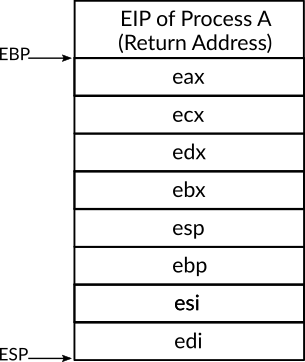
\includegraphics[width=0.35000\textwidth]{Figures/process-ch/Fig21092021_1.png}
\caption{Figure 2: The Stack After Executing the Instruction
\lstinline!pusha!}\label{fig:21092021_1}
\end{figure}
}

Let's assume that a process named \lstinline!A! was running and a system
timer interrupt occurred which caused process \lstinline!A! to suspend
and \lstinline!isr_32! to start, as we have mentioned earlier,
\lstinline!isr_32! will be called as a normal routine and the calling
convention will be followed by the processor. Figure
\protect\hyperlink{fig:21092021_1}{2} shows the stack at the time after
executing \lstinline!pusha! in \lstinline!isr_32!. As you can see, the
context of process \lstinline!A! is on the stack, for example, to reach
the value of \lstinline!ESI! which was stored right before the process
\lstinline!A! has been suspended, we can do that by referring to the
memory address \lstinline!ESP + 4! \footnote{If a new stack frame is
  created once \lstinline!isr_32! starts then also \lstinline!EBP! can
  be used as a base address but with different offset than \lstinline!4!
  of course as we have explained earlier in chapter \ref{ch-x86}. I
  didn't initialize a new stack frame here and in all other places to
  get a shorter code.}, since the current \lstinline!ESP! stores the
memory address of the top of the stack, the size of the value of
\lstinline!EDI! (and all other registers) is \lstinline!4! bytes and the
value of \lstinline!ESI! is next to the top of the stack.

The same technique can be used with any value in stack. As you may have
noticed in the figure, that the return address to where process
\lstinline!A! suspended is stored in the stack, and that's due to the
calling convention which requires the return address of the caller to be
stored in the stack so we can return to it, as you can see, here, the
process \lstinline!A! was considered as the caller and
\lstinline!isr_32! as the callee. So, to obtain the value of process
\lstinline!A!'s return address, we can do that simply by reading the
value in \lstinline!esp + 32!, and that exactly what we have done in the
third step of \lstinline!isr_32! code, we first read this value and then
push it into the stack so the function \lstinline!scheduler! can receive
it as the first parameter.

The fourth and fifth steps are simple, in the fourth step we call the
function \lstinline!scheduler! which we have already discussed, after
the function \lstinline!scheduler! returns, we need to tell PIC that we
finished the handling of an \lstinline!IRQ! by sending end of interrupt
command to the \lstinline!PIC! and that's what is performed in the fifth
step, we have already discussed sending end of interrupt command to PIC
in chapter \ref{ch-progenitor}.

The final thing to do after choosing the next process and performing the
context switching is to give a CPU time for the code of the next
process. This is usually performed by jumping to the memory address in
which the selected process where suspended. There are multiple ways to
do that, the way which we have used in 539kernel is to exploit the
calling convention, again.

As we have mentioned before, the return address to the caller is stored
in the stack, in our previous example, the return address to process
\lstinline!A! was stored in the stack right before the values of process
\lstinline!A! context which have been pushed by the instruction
\lstinline!pusha!. When a routine returns by using the instruction
\lstinline!ret! or \lstinline!iret!, this address will be jumped to, we
exploit this fact to make the next process runs after \lstinline!isr_32!
finishes instead of process \lstinline!A!, this is too simple to be
done, the return address of process \lstinline!A! should be removed from
the stack and in its position in the stack the resume point of the next
process is pushed, that's what we do in the sixth step of
\lstinline!isr_32!.

First we remove all values that we have pushed on the stack while
running \lstinline!isr_32!, this is performed by just adding
\lstinline!40! to the current value of \lstinline!ESP!, we have already
discussed this method of removing values from the stack, why adding
\lstinline!40!? You may ask. The number of values that have been pushed
by the instruction \lstinline!pusha! is \lstinline!8! values, each one
of them of size \lstinline!4! bytes (\lstinline!32-bit!), that means the
total size of them is \lstinline!4 * 8 = 32!. Also, we have pushed the
value of \lstinline!EIP! which also has the size of \lstinline!4! bytes,
so, until now the total size of pushed items in \lstinline!isr_32! is
\lstinline!32 + 4 = 36! and these are all what we have pushed in
purpose, we also need to remove the return address which has been pushed
into the stack before calling \lstinline!isr_32!, the size of memory
addresses in \lstinline!32-bit! architecture is \lstinline!4! bytes
(\lstinline!32-bit!), that means \lstinline!36 + 4 = 40! bytes should be
removed from the stack to ensure that we remove all pushed values with
the return address or process \lstinline!A!.

After that, we simply push the memory address of the function
\lstinline!run_next_process!. In the seventh step, the routine
\lstinline!isr_32! returns indicating that handling an interrupt has
been completed, but instead of returning to the suspended code before
calling the interrupt handler, the code of the function
\lstinline!run_next_process! will be called, which is, as we have seen,
enables the interrupts again and jumps to the resume point of the next
process. In this way, we have got a basic multitasking!

\subsection{Running Processes}\label{running-processes}

In our current environment, we will not be able to test our process
management by using the normal ways, I mean, we can't run a user-space
software to check if its process has been created and being scheduled or
not. Instead, we are going to create a number of processes by creating
their \lstinline!PCB!s via \lstinline!process_create! function, and
their code will be defined as functions in our kernel, the memory
address of these functions will be considered as the starting point of
the process. Our goal of doing that is just to test that our code of
process management is running well. All code of this section will be in
\lstinline!main.c! unless otherwise is mentioned. First, we define
prototypes for four functions, each one of them represents a separate
process, imaging them as a normal use-space software. These prototypes
should be defined before \lstinline!kernel_main!.

\begin{lstlisting}[language=C]
void processA();
void processB();
void processC();
void processD();
\end{lstlisting}

Inside \lstinline!kernel_main!, we define four local variables. Each one
of them represents the PCB of one process.

\begin{lstlisting}[language=C]
    process_t p1, p2, p3, p4;
\end{lstlisting}

Before the infinite loop of \lstinline!kernel_main! we create the four
processes in the system by using the function \lstinline!process_create!
as the following.

\begin{lstlisting}[language=C]
    process_create( &processA, &p1 );
    process_create( &processB, &p2 );
    process_create( &processC, &p3 );
    process_create( &processD, &p4 );
\end{lstlisting}

The code of the processes is the following.

\begin{lstlisting}[language=C]
void processA()
{
    print( "Process A," );

    while ( 1 )
        asm( "mov $5390, %eax" );
}

void processB()
{
    print( "Process B," );

    while ( 1 )
        asm( "mov $5391, %eax" );
}

void processC()
{
    print( "Process C," );

    while ( 1 )
        asm( "mov $5392, %eax" );
}

void processD()
{
    print( "Process D," );

    while ( 1 )
        asm( "mov $5393, %eax" );
}
\end{lstlisting}

Each process starts by printing its name, then, an infinite loop starts
which keeps setting a specific value in the register \lstinline!EAX!. To
check whether multitasking is working fine, we can add the following
lines the beginning of the function \lstinline!scheduler! in
\lstinline!scheduler.c!.

\begin{lstlisting}[language=C]
    print( " EAX = " );
    printi( eax );
\end{lstlisting}

Each time the scheduler starts, it prints the value of \lstinline!EAX!
of the suspended process. When we run the kernel, each process is going
to start by printing its name and before a process starts executing the
value of \lstinline!EAX! of the previous process will be shown.
Therefore, you will see a bunch of following texts
\lstinline!EAX = 5390!, \lstinline!EAX = 5391!, \lstinline!EAX = 5392!
and \lstinline!EAX = 5393! keep showing on the screen which indicates
that the process, \lstinline!A! for example in case
\lstinline!EAX = 5390! is shown, was running and it has been suspended
now to run the next one and so on.

\subsection{\texorpdfstring{Finishing up Version
\texttt{T}}{Finishing up Version T}}\label{finishing-up-version-t}

And we have got version \lstinline!T! of 539kernel which provides us a
basic process management subsystem. The last piece to be presented is
the \lstinline!Makefile! to compile the whole code.

\begin{lstlisting}[language=make]
ASM = nasm
CC = gcc
BOOTSTRAP_FILE = bootstrap.asm 
INIT_KERNEL_FILES = starter.asm
KERNEL_FILES = main.c
KERNEL_FLAGS = -Wall -m32 -c -ffreestanding -fno-asynchronous-unwind-tables -fno-pie
KERNEL_OBJECT = -o kernel.elf

build: $(BOOTSTRAP_FILE) $(KERNEL_FILE)
    $(ASM) -f bin $(BOOTSTRAP_FILE) -o bootstrap.o
    $(ASM) -f elf32 $(INIT_KERNEL_FILES) -o starter.o 
    $(CC) $(KERNEL_FLAGS) $(KERNEL_FILES) $(KERNEL_OBJECT)
    $(CC) $(KERNEL_FLAGS) screen.c -o screen.elf
    $(CC) $(KERNEL_FLAGS) process.c -o process.elf
    $(CC) $(KERNEL_FLAGS) scheduler.c -o scheduler.elf
    ld -melf_i386 -Tlinker.ld starter.o kernel.elf screen.elf process.elf scheduler.elf -o 539kernel.elf
    objcopy -O binary 539kernel.elf 539kernel.bin
    dd if=bootstrap.o of=kernel.img
    dd seek=1 conv=sync if=539kernel.bin of=kernel.img bs=512 count=8
    dd seek=9 conv=sync if=/dev/zero of=kernel.img bs=512 count=2046
    qemu-system-x86_64 -s kernel.img
\end{lstlisting}

Nothing new in here but compiling the new C files that we have added to
539kernel.
